%Capitulo 3, presentación 45
\definecolor{Red}{RGB}{100,10,10}
\definecolor{DarkGreen}{RGB}{10,100,10}
\begin{frame}{Busqueda "Deph-First"}
    Expandir el nodo no expandido más profundo
    \\
    \textcolor{Red}{\large{Implementación:}}
    \\
    \qquad\qquad\textcolor{DarkGreen}{\textit{fringe}} = Cola LIFO, es decir , poner el sucesor al frente
    \\
    \centering
    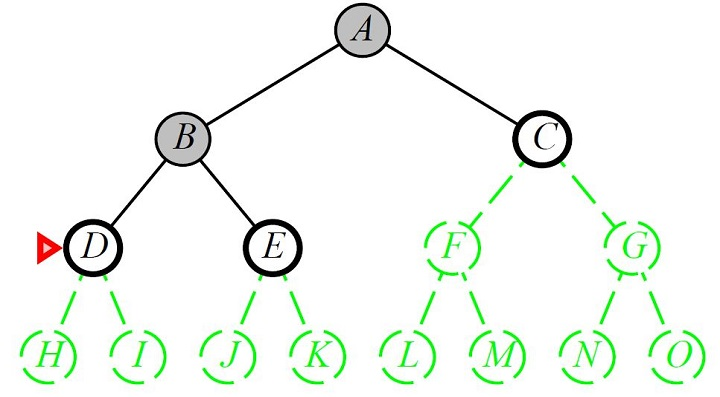
\includegraphics[scale=.5]{images/43_tree.JPG} 
\end{frame}